% GNUPLOT: LaTeX picture with Postscript
\begingroup
  \makeatletter
  \providecommand\color[2][]{%
    \GenericError{(gnuplot) \space\space\space\@spaces}{%
      Package color not loaded in conjunction with
      terminal option `colourtext'%
    }{See the gnuplot documentation for explanation.%
    }{Either use 'blacktext' in gnuplot or load the package
      color.sty in LaTeX.}%
    \renewcommand\color[2][]{}%
  }%
  \providecommand\includegraphics[2][]{%
    \GenericError{(gnuplot) \space\space\space\@spaces}{%
      Package graphicx or graphics not loaded%
    }{See the gnuplot documentation for explanation.%
    }{The gnuplot epslatex terminal needs graphicx.sty or graphics.sty.}%
    \renewcommand\includegraphics[2][]{}%
  }%
  \providecommand\rotatebox[2]{#2}%
  \@ifundefined{ifGPcolor}{%
    \newif\ifGPcolor
    \GPcolorfalse
  }{}%
  \@ifundefined{ifGPblacktext}{%
    \newif\ifGPblacktext
    \GPblacktexttrue
  }{}%
  % define a \g@addto@macro without @ in the name:
  \let\gplgaddtomacro\g@addto@macro
  % define empty templates for all commands taking text:
  \gdef\gplbacktext{}%
  \gdef\gplfronttext{}%
  \makeatother
  \ifGPblacktext
    % no textcolor at all
    \def\colorrgb#1{}%
    \def\colorgray#1{}%
  \else
    % gray or color?
    \ifGPcolor
      \def\colorrgb#1{\color[rgb]{#1}}%
      \def\colorgray#1{\color[gray]{#1}}%
      \expandafter\def\csname LTw\endcsname{\color{white}}%
      \expandafter\def\csname LTb\endcsname{\color{black}}%
      \expandafter\def\csname LTa\endcsname{\color{black}}%
      \expandafter\def\csname LT0\endcsname{\color[rgb]{1,0,0}}%
      \expandafter\def\csname LT1\endcsname{\color[rgb]{0,1,0}}%
      \expandafter\def\csname LT2\endcsname{\color[rgb]{0,0,1}}%
      \expandafter\def\csname LT3\endcsname{\color[rgb]{1,0,1}}%
      \expandafter\def\csname LT4\endcsname{\color[rgb]{0,1,1}}%
      \expandafter\def\csname LT5\endcsname{\color[rgb]{1,1,0}}%
      \expandafter\def\csname LT6\endcsname{\color[rgb]{0,0,0}}%
      \expandafter\def\csname LT7\endcsname{\color[rgb]{1,0.3,0}}%
      \expandafter\def\csname LT8\endcsname{\color[rgb]{0.5,0.5,0.5}}%
    \else
      % gray
      \def\colorrgb#1{\color{black}}%
      \def\colorgray#1{\color[gray]{#1}}%
      \expandafter\def\csname LTw\endcsname{\color{white}}%
      \expandafter\def\csname LTb\endcsname{\color{black}}%
      \expandafter\def\csname LTa\endcsname{\color{black}}%
      \expandafter\def\csname LT0\endcsname{\color{black}}%
      \expandafter\def\csname LT1\endcsname{\color{black}}%
      \expandafter\def\csname LT2\endcsname{\color{black}}%
      \expandafter\def\csname LT3\endcsname{\color{black}}%
      \expandafter\def\csname LT4\endcsname{\color{black}}%
      \expandafter\def\csname LT5\endcsname{\color{black}}%
      \expandafter\def\csname LT6\endcsname{\color{black}}%
      \expandafter\def\csname LT7\endcsname{\color{black}}%
      \expandafter\def\csname LT8\endcsname{\color{black}}%
    \fi
  \fi
    \setlength{\unitlength}{0.0500bp}%
    \ifx\gptboxheight\undefined%
      \newlength{\gptboxheight}%
      \newlength{\gptboxwidth}%
      \newsavebox{\gptboxtext}%
    \fi%
    \setlength{\fboxrule}{0.5pt}%
    \setlength{\fboxsep}{1pt}%
\begin{picture}(7200.00,5040.00)%
    \gplgaddtomacro\gplbacktext{%
      \csname LTb\endcsname%%
      \put(588,3706){\makebox(0,0)[r]{\strut{}-0.04}}%
      \csname LTb\endcsname%%
      \put(588,3953){\makebox(0,0)[r]{\strut{}-0.02}}%
      \csname LTb\endcsname%%
      \put(588,4199){\makebox(0,0)[r]{\strut{}0.00}}%
      \csname LTb\endcsname%%
      \put(588,4445){\makebox(0,0)[r]{\strut{}0.02}}%
      \csname LTb\endcsname%%
      \put(588,4692){\makebox(0,0)[r]{\strut{}0.04}}%
      \csname LTb\endcsname%%
      \put(896,3240){\makebox(0,0){\strut{}}}%
      \csname LTb\endcsname%%
      \put(1248,3240){\makebox(0,0){\strut{}}}%
      \csname LTb\endcsname%%
      \put(1600,3240){\makebox(0,0){\strut{}}}%
      \csname LTb\endcsname%%
      \put(1951,3240){\makebox(0,0){\strut{}}}%
      \csname LTb\endcsname%%
      \put(2303,3240){\makebox(0,0){\strut{}}}%
      \csname LTb\endcsname%%
      \put(2655,3240){\makebox(0,0){\strut{}}}%
      \put(1776,4774){\makebox(0,0){\strut{}$t = 0$}}%
    }%
    \gplgaddtomacro\gplfronttext{%
      \csname LTb\endcsname%%
      \put(-182,4199){\rotatebox{-270}{\makebox(0,0){\strut{}$\phi(t,r)$}}}%
    }%
    \gplgaddtomacro\gplbacktext{%
      \csname LTb\endcsname%%
      \put(2700,3706){\makebox(0,0)[r]{\strut{}}}%
      \csname LTb\endcsname%%
      \put(2700,3953){\makebox(0,0)[r]{\strut{}}}%
      \csname LTb\endcsname%%
      \put(2700,4199){\makebox(0,0)[r]{\strut{}}}%
      \csname LTb\endcsname%%
      \put(2700,4445){\makebox(0,0)[r]{\strut{}}}%
      \csname LTb\endcsname%%
      \put(2700,4692){\makebox(0,0)[r]{\strut{}}}%
      \csname LTb\endcsname%%
      \put(3008,3240){\makebox(0,0){\strut{}}}%
      \csname LTb\endcsname%%
      \put(3360,3240){\makebox(0,0){\strut{}}}%
      \csname LTb\endcsname%%
      \put(3712,3240){\makebox(0,0){\strut{}}}%
      \csname LTb\endcsname%%
      \put(4063,3240){\makebox(0,0){\strut{}}}%
      \csname LTb\endcsname%%
      \put(4415,3240){\makebox(0,0){\strut{}}}%
      \csname LTb\endcsname%%
      \put(4767,3240){\makebox(0,0){\strut{}}}%
      \put(3888,4774){\makebox(0,0){\strut{}$t = 0.5\times10^{3}\Delta t$}}%
    }%
    \gplgaddtomacro\gplfronttext{%
    }%
    \gplgaddtomacro\gplbacktext{%
      \csname LTb\endcsname%%
      \put(4812,3706){\makebox(0,0)[r]{\strut{}}}%
      \csname LTb\endcsname%%
      \put(4812,3953){\makebox(0,0)[r]{\strut{}}}%
      \csname LTb\endcsname%%
      \put(4812,4199){\makebox(0,0)[r]{\strut{}}}%
      \csname LTb\endcsname%%
      \put(4812,4445){\makebox(0,0)[r]{\strut{}}}%
      \csname LTb\endcsname%%
      \put(4812,4692){\makebox(0,0)[r]{\strut{}}}%
      \csname LTb\endcsname%%
      \put(5120,3240){\makebox(0,0){\strut{}}}%
      \csname LTb\endcsname%%
      \put(5472,3240){\makebox(0,0){\strut{}}}%
      \csname LTb\endcsname%%
      \put(5824,3240){\makebox(0,0){\strut{}}}%
      \csname LTb\endcsname%%
      \put(6175,3240){\makebox(0,0){\strut{}}}%
      \csname LTb\endcsname%%
      \put(6527,3240){\makebox(0,0){\strut{}}}%
      \csname LTb\endcsname%%
      \put(6879,3240){\makebox(0,0){\strut{}}}%
      \put(6000,4774){\makebox(0,0){\strut{}$t = 1.0\times10^{3}\Delta t$}}%
    }%
    \gplgaddtomacro\gplfronttext{%
    }%
    \gplgaddtomacro\gplbacktext{%
      \csname LTb\endcsname%%
      \put(588,2228){\makebox(0,0)[r]{\strut{}-0.04}}%
      \csname LTb\endcsname%%
      \put(588,2475){\makebox(0,0)[r]{\strut{}-0.02}}%
      \csname LTb\endcsname%%
      \put(588,2721){\makebox(0,0)[r]{\strut{}0.00}}%
      \csname LTb\endcsname%%
      \put(588,2967){\makebox(0,0)[r]{\strut{}0.02}}%
      \csname LTb\endcsname%%
      \put(588,3214){\makebox(0,0)[r]{\strut{}0.04}}%
      \csname LTb\endcsname%%
      \put(896,1762){\makebox(0,0){\strut{}}}%
      \csname LTb\endcsname%%
      \put(1248,1762){\makebox(0,0){\strut{}}}%
      \csname LTb\endcsname%%
      \put(1600,1762){\makebox(0,0){\strut{}}}%
      \csname LTb\endcsname%%
      \put(1951,1762){\makebox(0,0){\strut{}}}%
      \csname LTb\endcsname%%
      \put(2303,1762){\makebox(0,0){\strut{}}}%
      \csname LTb\endcsname%%
      \put(2655,1762){\makebox(0,0){\strut{}}}%
      \put(1776,3296){\makebox(0,0){\strut{}$t = 1.5\times10^{3}\Delta t$}}%
    }%
    \gplgaddtomacro\gplfronttext{%
      \csname LTb\endcsname%%
      \put(-182,2721){\rotatebox{-270}{\makebox(0,0){\strut{}$\phi(t,r)$}}}%
    }%
    \gplgaddtomacro\gplbacktext{%
      \csname LTb\endcsname%%
      \put(2700,2228){\makebox(0,0)[r]{\strut{}}}%
      \csname LTb\endcsname%%
      \put(2700,2475){\makebox(0,0)[r]{\strut{}}}%
      \csname LTb\endcsname%%
      \put(2700,2721){\makebox(0,0)[r]{\strut{}}}%
      \csname LTb\endcsname%%
      \put(2700,2967){\makebox(0,0)[r]{\strut{}}}%
      \csname LTb\endcsname%%
      \put(2700,3214){\makebox(0,0)[r]{\strut{}}}%
      \csname LTb\endcsname%%
      \put(3008,1762){\makebox(0,0){\strut{}}}%
      \csname LTb\endcsname%%
      \put(3360,1762){\makebox(0,0){\strut{}}}%
      \csname LTb\endcsname%%
      \put(3712,1762){\makebox(0,0){\strut{}}}%
      \csname LTb\endcsname%%
      \put(4063,1762){\makebox(0,0){\strut{}}}%
      \csname LTb\endcsname%%
      \put(4415,1762){\makebox(0,0){\strut{}}}%
      \csname LTb\endcsname%%
      \put(4767,1762){\makebox(0,0){\strut{}}}%
      \put(3888,3296){\makebox(0,0){\strut{}$t = 2.0\times10^{3}\Delta t$}}%
    }%
    \gplgaddtomacro\gplfronttext{%
    }%
    \gplgaddtomacro\gplbacktext{%
      \csname LTb\endcsname%%
      \put(4812,2228){\makebox(0,0)[r]{\strut{}}}%
      \csname LTb\endcsname%%
      \put(4812,2475){\makebox(0,0)[r]{\strut{}}}%
      \csname LTb\endcsname%%
      \put(4812,2721){\makebox(0,0)[r]{\strut{}}}%
      \csname LTb\endcsname%%
      \put(4812,2967){\makebox(0,0)[r]{\strut{}}}%
      \csname LTb\endcsname%%
      \put(4812,3214){\makebox(0,0)[r]{\strut{}}}%
      \csname LTb\endcsname%%
      \put(5120,1762){\makebox(0,0){\strut{}}}%
      \csname LTb\endcsname%%
      \put(5472,1762){\makebox(0,0){\strut{}}}%
      \csname LTb\endcsname%%
      \put(5824,1762){\makebox(0,0){\strut{}}}%
      \csname LTb\endcsname%%
      \put(6175,1762){\makebox(0,0){\strut{}}}%
      \csname LTb\endcsname%%
      \put(6527,1762){\makebox(0,0){\strut{}}}%
      \csname LTb\endcsname%%
      \put(6879,1762){\makebox(0,0){\strut{}}}%
      \put(6000,3296){\makebox(0,0){\strut{}$t = 2.5\times10^{3}\Delta t$}}%
    }%
    \gplgaddtomacro\gplfronttext{%
    }%
    \gplgaddtomacro\gplbacktext{%
      \csname LTb\endcsname%%
      \put(588,750){\makebox(0,0)[r]{\strut{}-0.04}}%
      \csname LTb\endcsname%%
      \put(588,997){\makebox(0,0)[r]{\strut{}-0.02}}%
      \csname LTb\endcsname%%
      \put(588,1243){\makebox(0,0)[r]{\strut{}0.00}}%
      \csname LTb\endcsname%%
      \put(588,1489){\makebox(0,0)[r]{\strut{}0.02}}%
      \csname LTb\endcsname%%
      \put(588,1736){\makebox(0,0)[r]{\strut{}0.04}}%
      \csname LTb\endcsname%%
      \put(896,284){\makebox(0,0){\strut{}$0$}}%
      \csname LTb\endcsname%%
      \put(1248,284){\makebox(0,0){\strut{}$10$}}%
      \csname LTb\endcsname%%
      \put(1600,284){\makebox(0,0){\strut{}$20$}}%
      \csname LTb\endcsname%%
      \put(1951,284){\makebox(0,0){\strut{}$30$}}%
      \csname LTb\endcsname%%
      \put(2303,284){\makebox(0,0){\strut{}$40$}}%
      \csname LTb\endcsname%%
      \put(2655,284){\makebox(0,0){\strut{}$50$}}%
      \put(1776,1818){\makebox(0,0){\strut{}$t = 3.0\times10^{3}\Delta t$}}%
    }%
    \gplgaddtomacro\gplfronttext{%
      \csname LTb\endcsname%%
      \put(-182,1243){\rotatebox{-270}{\makebox(0,0){\strut{}$\phi(t,r)$}}}%
      \put(1775,-46){\makebox(0,0){\strut{}$r$}}%
    }%
    \gplgaddtomacro\gplbacktext{%
      \csname LTb\endcsname%%
      \put(2700,750){\makebox(0,0)[r]{\strut{}}}%
      \csname LTb\endcsname%%
      \put(2700,997){\makebox(0,0)[r]{\strut{}}}%
      \csname LTb\endcsname%%
      \put(2700,1243){\makebox(0,0)[r]{\strut{}}}%
      \csname LTb\endcsname%%
      \put(2700,1489){\makebox(0,0)[r]{\strut{}}}%
      \csname LTb\endcsname%%
      \put(2700,1736){\makebox(0,0)[r]{\strut{}}}%
      \csname LTb\endcsname%%
      \put(3008,284){\makebox(0,0){\strut{}$0$}}%
      \csname LTb\endcsname%%
      \put(3360,284){\makebox(0,0){\strut{}$10$}}%
      \csname LTb\endcsname%%
      \put(3712,284){\makebox(0,0){\strut{}$20$}}%
      \csname LTb\endcsname%%
      \put(4063,284){\makebox(0,0){\strut{}$30$}}%
      \csname LTb\endcsname%%
      \put(4415,284){\makebox(0,0){\strut{}$40$}}%
      \csname LTb\endcsname%%
      \put(4767,284){\makebox(0,0){\strut{}$50$}}%
      \put(3888,1818){\makebox(0,0){\strut{}$t = 3.5\times10^{3}\Delta t$}}%
    }%
    \gplgaddtomacro\gplfronttext{%
      \csname LTb\endcsname%%
      \put(3887,-46){\makebox(0,0){\strut{}$r$}}%
    }%
    \gplgaddtomacro\gplbacktext{%
      \csname LTb\endcsname%%
      \put(4812,750){\makebox(0,0)[r]{\strut{}}}%
      \csname LTb\endcsname%%
      \put(4812,997){\makebox(0,0)[r]{\strut{}}}%
      \csname LTb\endcsname%%
      \put(4812,1243){\makebox(0,0)[r]{\strut{}}}%
      \csname LTb\endcsname%%
      \put(4812,1489){\makebox(0,0)[r]{\strut{}}}%
      \csname LTb\endcsname%%
      \put(4812,1736){\makebox(0,0)[r]{\strut{}}}%
      \csname LTb\endcsname%%
      \put(5120,284){\makebox(0,0){\strut{}$0$}}%
      \csname LTb\endcsname%%
      \put(5472,284){\makebox(0,0){\strut{}$10$}}%
      \csname LTb\endcsname%%
      \put(5824,284){\makebox(0,0){\strut{}$20$}}%
      \csname LTb\endcsname%%
      \put(6175,284){\makebox(0,0){\strut{}$30$}}%
      \csname LTb\endcsname%%
      \put(6527,284){\makebox(0,0){\strut{}$40$}}%
      \csname LTb\endcsname%%
      \put(6879,284){\makebox(0,0){\strut{}$50$}}%
      \put(6000,1818){\makebox(0,0){\strut{}$t = 4.0\times10^{3}\Delta t$}}%
    }%
    \gplgaddtomacro\gplfronttext{%
      \csname LTb\endcsname%%
      \put(5999,-46){\makebox(0,0){\strut{}$r$}}%
    }%
    \gplbacktext
    \put(0,0){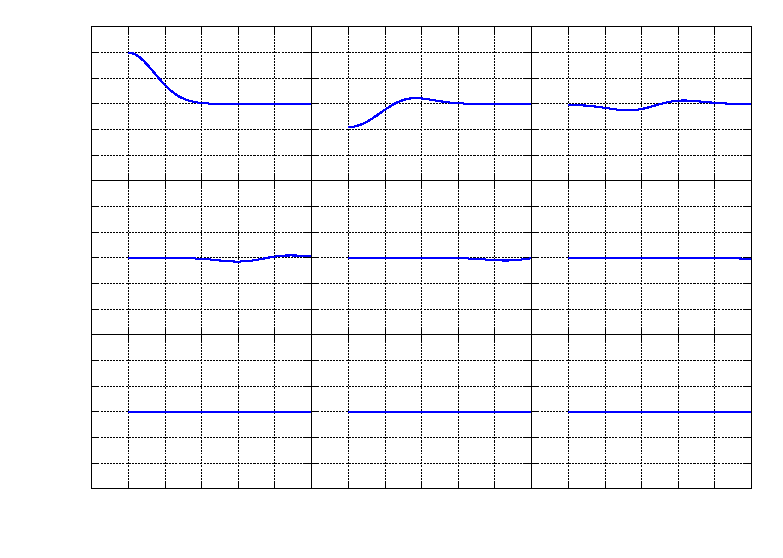
\includegraphics{scalarfield_weak}}%
    \gplfronttext
  \end{picture}%
\endgroup
